\tikzset{every picture/.style={line width=0.75pt}} %set default line width to 0.75pt         
 
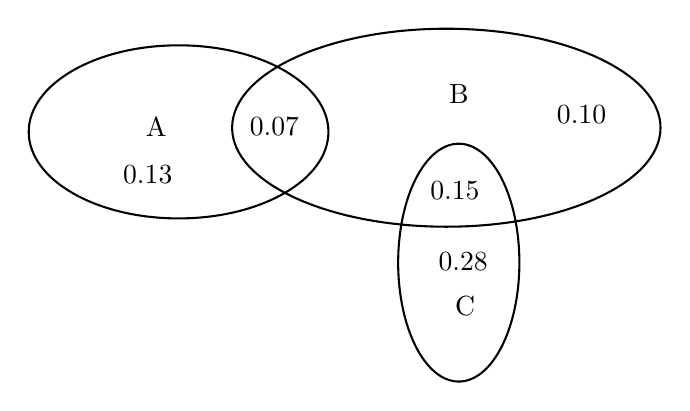
\begin{tikzpicture}[x=0.75pt,y=0.75pt,yscale=-1,xscale=1] 
%uncomment if require: \path (0,300); %set diagram left start at 0, and has height of 300 
 
%Shape: Ellipse [id:dp6642498322540047]  
\draw   (106,103.3) .. controls (106,80.27) and (138.33,61.6) .. (178.2,61.6) .. controls (218.07,61.6) and (250.4,80.27) .. (250.4,103.3) .. controls (250.4,126.33) and (218.07,145) .. (178.2,145) .. controls (138.33,145) and (106,126.33) .. (106,103.3) -- cycle ; 
%Shape: Ellipse [id:dp7872013385898509]  
\draw   (204,101.3) .. controls (204,74.96) and (250.2,53.6) .. (307.2,53.6) .. controls (364.2,53.6) and (410.4,74.96) .. (410.4,101.3) .. controls (410.4,127.64) and (364.2,149) .. (307.2,149) .. controls (250.2,149) and (204,127.64) .. (204,101.3) -- cycle ; 
%Shape: Ellipse [id:dp8712639118089818]  
\draw   (313.2,109) .. controls (329.33,109) and (342.4,134.65) .. (342.4,166.3) .. controls (342.4,197.95) and (329.33,223.6) .. (313.2,223.6) .. controls (297.07,223.6) and (284,197.95) .. (284,166.3) .. controls (284,134.65) and (297.07,109) .. (313.2,109) -- cycle ; 
 
% Text Node 
\draw (161,95) node [anchor=north west][inner sep=0.75pt]   [align=left] {A}; 
% Text Node 
\draw (307,79) node [anchor=north west][inner sep=0.75pt]   [align=left] {B}; 
% Text Node 
\draw (310,181) node [anchor=north west][inner sep=0.75pt]   [align=left] {C}; 
% Text Node 
\draw (150,118) node [anchor=north west][inner sep=0.75pt]   [align=left] {0.13}; 
% Text Node 
\draw (211,95) node [anchor=north west][inner sep=0.75pt]   [align=left] {0.07}; 
% Text Node 
\draw (298,126) node [anchor=north west][inner sep=0.75pt]   [align=left] {0.15}; 
% Text Node 
\draw (359,89) node [anchor=north west][inner sep=0.75pt]   [align=left] {0.10}; 
% Text Node 
\draw (302,160) node [anchor=north west][inner sep=0.75pt]   [align=left] {0.28\\}; 
 
 
\end{tikzpicture}
